\section{Tickets}
\label{sec:tickets}

The HOPR protocol makes use of a custom micropayment scheme to process its incentives. This section focuses on the utilized micro-payment scheme and serves as a building block for section \ref{sec:incentives}.

Incentives are handled by a structure called \textit{tickets} that is inspired by payment channels as well as probabilistic payments and allows nodes to issue asset transfers without requiring each time an on-chain interaction. Tickets are sent locked and get unlocked afterwards, i. e. after proving that a packet has been relayed. Nodes who receive a locked ticket are able to validate its validity. Once a node has received the required cryptographic material to unlock the ticket, it is able to claim the incentive by submitting the ticket to the smart contract.

\begin{figure}[H]
    \centering
    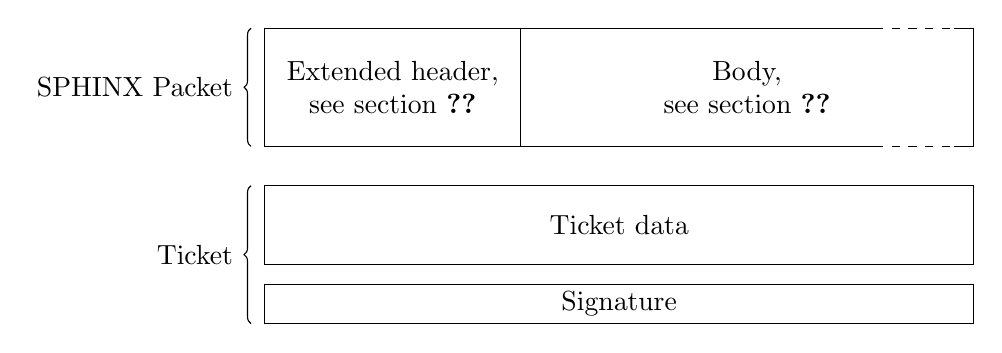
\begin{tikzpicture}[every text node part/.style={align=center}]
        \def\width{9}
        \def\headerWidth{9}
        \def\headerHeight{1.5}
        \def\headerOffset{3.25}
        \def\dashOffset{4.5}
        \def\dashWidth{1}

        \def\ticketDataHeight{1}
        \def\ticketSignatureHeight{0.5}

        \draw[decoration={brace,raise=5pt,mirror},decorate] (0,0) -- node[left=8pt] {SPHINX Packet} (0,-\headerHeight);

        \draw (0,0) rectangle (\headerOffset,-\headerHeight) node [midway] {Extended header,\\see section \ref{sec:incentives:proofofrelay}};
        \path [shape=rectangle] (\headerOffset,0) rectangle (\headerWidth,-\headerHeight) node [midway] {Body,\\see section \ref{sec:sphinx:payload}};

        \draw (\headerOffset+\dashOffset,-\headerHeight) -- (\headerOffset,-\headerHeight) -- (\headerOffset,0) -- (\headerOffset+\dashOffset,0);

        \draw [dashed] (\headerOffset+\dashOffset,0) -- (\headerOffset+\dashOffset+\dashWidth,0);
        \draw [dashed] (\headerOffset+\dashOffset,-\headerHeight) -- (\headerOffset+\dashOffset+\dashWidth,-\headerHeight);

        \draw (\headerOffset+\dashOffset+\dashWidth,-\headerHeight) -- (\headerWidth,-\headerHeight) -- (\headerWidth,0) -- (\headerOffset+\dashOffset+\dashWidth,0);

        \begin{scope}[shift={(0,-\headerHeight-0.5)}]
            \def\padding{0.25}

            \draw[decoration={brace,raise=5pt,mirror},decorate] (0,0) -- node[left=8pt] {Ticket} (0,-\ticketDataHeight-\padding-\ticketSignatureHeight);

            \draw (0,0) rectangle (\headerWidth,-\ticketDataHeight) node [midway] {Ticket data};

            \draw (0,-\ticketDataHeight-\padding) rectangle (\headerWidth,-\ticketDataHeight-\ticketSignatureHeight-\padding) node [midway] {Signature};
        \end{scope}
    \end{tikzpicture}
    \caption{Schematic overview of a mixnet packet that is sent together with a ticket.}
\end{figure}

\subsection{Ticket Issuance}
\label{sec:tickets:issuance}

Before a node can issue tickets to another node, it needs to lock funds on-chain to cover the cost of current and future tickets. Locking funds is considered equivalent to staking tokens in the HOPR network as it allows the node to create mixnet packets and act as relayer. By locking tokens in the smart contract, the node creates a unidirectional payment channel towards the recipient and is thus able to prove its eligibility to issue tickets to the recipient.

As ticket issuance happens without any interaction with the blockchain, it is the duty of the receiving node to validate whether sufficient tokens are locked on-chain and to keep track of previously issued tickets. If there is no on-chain record of any locked funds or if the sum of the received tickets exceeds the amount of tokens locked on-chain, the recipient should refuse the ticket.\footnote{TODO: Explain the consequences of ignoring this.}

Tickets are sent together with a mixnet packet and include the incentive for processing and forwarding the packet to the next downstream node. To meet the \lcnameref{sec:intro:securitygoals},\footnote{TODO: Further specify how and which security goals are met here.} neither issuance nor redemption must be linkable to the creation or processing of mixnet packets. Therefore, each ticket is given a winning probability. This means that all tickets produce a claimable incentive and winning tickets mitigate the lack of incentives for losing tickets.\footnote{TODO: Expand on this concept to show expected break-even times and variance of different winning probabilities.} By reducing on-chain interactions, this approach not only provides privacy, it also significantly reduces transaction costs.

When issuing a ticket, the issuer picks a winning probability $winProb > 0$ and starts creating the data structure $ticketData$ by setting the intended value $value$ through

$$ ticketData.value := \frac{value(ticket)}{winProb} $$

Note that the ticket issuer should not choose $winProb$ too low as the recipient might refuse the ticket due to inappropriate winning probability.

\begin{figure}[H]
    \centering
    \begin{tabular}{c|l|c|c|}
        \cline{2-4}
                                                    & \textbf{Value}                                    & \textbf{Ethereum datatype} & \textbf{size (in bytes)} \\
        \cline{2-4}
        \noalign{\smallskip}
        \cline{2-4}
        \multirow{7}{*}{\rotatebox{90}{TicketData}} & \nameref{sec:tickets:issuance:recipient}          & address                    & 20 bytes                 \\
                                                    & \nameref{sec:tickets:issuance:challenge}          & bytes32                    & 32 bytes                 \\
                                                    & \nameref{sec:tickets:issuance:ticketepoch}        & uint256                    & 32 bytes                 \\
                                                    & \nameref{sec:tickets:issuance:ticketvalue}        & uint256                    & 32 bytes                 \\
                                                    & \nameref{sec:tickets:issuance:winningprobability} & uint256                    & 32 bytes                 \\
                                                    & \nameref{sec:tickets:issuance:ticketindex}        & uint256                    & 32 bytes                 \\
                                                    & \nameref{sec:tickets:issuance:channelepoch}       & uint256                    & 32 bytes                 \\
        \cline{2-4}
        \noalign{\smallskip}

        \cline{2-4}
        \multirow{3}{*}{\rotatebox{90}{Sig}}        & Signature $r$                                     & bytes32                    & 32 bytes                 \\
                                                    & Signature $s$                                     & bytes32                    & 32 bytes                 \\
                                                    & Recovery value $v$                                & uint8                      & 1 byte                   \\
        \cline{2-4}
    \end{tabular}
    \caption{Structure of a ticket.}
    \label{fig:ticketdata}
\end{figure}

\paragraph{Recipient}
\label{sec:tickets:issuance:recipient}

The Ethereum address of the recipient, derived from the recipient's public key. This confines the ticket to one specific payment channel, the one from ticket issuer to ticket recipient. Note that Ethereum addresses are computed as

$$ ethAddr: pubKey \in \{ 0,1 \}^{64} \mapsto \mathsf{keccak256}( pubKey).\mathsf{slice}(12,32)$$

(the last 20 bytes of the keccak256 hash of the uncompressed ECDSA public key).

\paragraph{Challenge}
\label{sec:tickets:issuance:challenge}

Tickets are issued locked, hence the embedded incentive is not yet claimable by the ticket recipient, although the ticket's validity can be verified. Locked means that the ticket states a challenge which needs to be solved before being able to claim the embedded incentive. This mechanism servers as a building block for \lcnameref{sec:incentives:proofofrelay}.

\paragraph{Ticket epoch}
\label{sec:tickets:issuance:ticketepoch}

Ticket redemption relies on providing the value $opening$\footnote{TODO: Properly introduce this value} to a series of commitments that have previously been stored on-chain by the ticket recipient. To ensure that the recipient is always able to compute the opening to a commitment, there is the opportunity to renew the on-chain commitment. As this allows the recipient to change the entropy used to determine whether a ticket is a winner (see Section \ref{sec:incentives:commitment}, the smart contract stores a counter that increases on every renewal and the ticket issuer signs the current value. This ensures that each commitment renewal invalidates all issued but unredeemed tickets.

\paragraph{Ticket value}
\label{sec:tickets:issuance:ticketvalue}

The ticket value is given by the intended $value$ divided by the winning probability $winProb$ in the base unit of the token, which is $10^{-8}$. Hence, sending $1$ HOPR with a winning probability of $1$ leads to $ticket.value = 10^8$.

\paragraph{Winning probability}
\label{sec:tickets:issuance:winningprobability}

The proportion of tickets which lead to an actual payout is determined by their winning probability. To prevent from issues resulting from roundings, $ticketData$ includes the inverse winning probability that is normalized with the common base of Ethereum, which is $2^{256} - 1$. Hence,

$$ ticketData.invWinProb := winProb * (2^{256} -1)$$

\paragraph{Ticket index}
\label{sec:tickets:issuance:ticketindex}

Each ticket is labeled by an incrementing serial number named the ticket index, $i$, whose current value is stored in the smart contract. Whenever a ticket is redeemed, the stored value is updated to the value given by the redeemed ticket. This invalidates all tickets with index $i' \le i$. This is necessary to ensure each ticket is valid exactly once. Since ticket issuance does not change the value stored in the smart contract and tickets with unchanged ticket index are worthless, it is the duty of the ticket recipient to ensure that the ticket index correctly increments, and to refuse tickets with an incorrect index.

\paragraph{Channel epoch}
\label{sec:tickets:issuance:channelepoch}

Payment channels can run through multiple \textit{open} and \textit{close} sequences (see Section \ref{sec:incentives:channels} for more information). To ensure that tickets from previous channel incarnations lose their value once the channel is reopened, tickets include the current channel epoch counter and the smart contract considers the ticket invalid if the signed channel epoch does not match the stored channel epoch.

\paragraph{Signature}
\label{sec:tickets:issuance:signature}

As a last step, the issuer creates a signature over the hash of the ticket with

\begin{multline*}
    ticketHash = keccak256 (recipient \ || \ ethAddr(challenge) \ || \ ticketEpoch \ ||  \\
    amount \ || \ invWinProb \ || \ index \ || \ channelEpoch)
\end{multline*}

yielding the ticket $t = (ticketData, Sig_{Issuer}(ticketHash))$.
\subsection{Ticket Validation}
\label{sec:tickets:validation}

Tickets are used to convince their recipient that they will receive the promised incentive once the challenge is solved. As ticket issuance happens without any on-chain interaction, it is the duty of the recipient to decide whether to accept or refuse a ticket.

Ticket validation runs through two states: receiving the ticket without knowing the response to the given challenge stated as $ticket.challenge$, \lcnameref{sec:tickets:validation:locked}, and once the response is known, \lcnameref{sec:tickets:validation:unlocked}.

\paragraph{Validation of Locked Tickets}
\label{sec:tickets:validation:locked}

Since there is no response to the stated challenge, the node cannot determine whether the ticket is going to be a winner nor claim it on-chain to receive the incentives. Nevertheless, the node can use the embedded information to validate the ticket economically. Therefore, the node first extracts the winning probability as

$$ticket.winProb = \frac{ticket.invWinProb}{2^{256} - 1} $$

which leads to $ value(ticket) = ticket.value \cdot ticket.invWinProb $. If the node considers $value(ticket)$ incorrect, i.e., because it does match the expected amount, or if winning probability is set too high or too low, it should refuse the ticket.

As ticket issuance happens without any on-chain interaction, there is no guarantee that the payment channel has sufficient locked tokens to pay a winning ticket, or indeed that the channel exists at all. Therefore, the recipient must check both of these before considering a ticket valid. In addition, there could be previous tickets, denoted as $stored$, which have not yet been redeemed. Hence, the recipient needs to check that

$$ channel.amount \le value(ticket) + \sum_{t \ \in \ stored} value(t)$$

In addition, as tickets are issued with an incremental serial number, the recipient must check that $ticket_i.index > \max(ticket_{i-1}.index,0)$ and refuse the ticket otherwise.

It remains to be shown that the ticket issuer indeed knows any $response$ which solve $ticket.challenge$. This is especially relevant if the ticket issuer was given the challenge by a third party, i.e., the creator of a mixnet packet. This will be covered in Section \ref{sec:incentives:proofofrelay}.

\paragraph{Validation of Unlocked Tickets}
\label{sec:tickets:validation:unlocked}

Once the $response$ to $ticket.challenge$ is known, i.e., after receiving a packet acknowledgement, the node can determine whether the ticket is going to be a winner. To check this, the node first computes the next $opening$ to the current value $commitment$\footnote{TODO: Properly define this value} stored in the smart contract and checks whether

$$ \mathsf{keccak256} ( \ \mathsf{keccak256}(ticketData) \ || \ solution \ || \ opening \ ) < ticket.winProb $$

If true, the node can consider the ticket to be a winner and store it for later use. If the ticket turns out to be a loser, there is no added value to it and the node can safely drop it. Note that losing tickets are an integral part of the mechanism and do not reduce the average payout to the ticket recipient. This is because $value(ticket)$ is given by the expected value and hence the asymptotic payout does not change.
\subsection{Ticket Redemption}
\label{sec:tickets:redemption}

After running through the validations of the previous section, the node $n$ ends up with a set of stored tickets which it considers to be a win, hence

$$ stored := \{ t \in Tickets \ | \ isWinner(t) \land t.recipient = n \}$$

Each ticket $t$ is given a  \lcnameref{sec:tickets:issuance:ticketindex}, which means tickets need to be redeemed in order which is why the node first creates an ordered set $ordered$ out of the set $tickets$ and proceeds with the first ticket.

Redemption means that the node now proves for each $t \in stored$ one-by-one to the smart contract that $t$ is indeed a win. If successful, the smart contract transfers the stated incentives to the account of the node, see paragraph \lcnameref{sec:tickets:redemption:assettransfer}.

In contrast to ticket recipients, the smart contract considers a ticket only valid if the redeemer is able to provide a $response$ that solves $ticket.challenge$ and a value $opening$ that opens the most recent $commitment$ stored on-chain. Note that the smart contract thereby acts as a trusted third party that forces the node reveal additional cryptographic material despite the signature of the ticket is valid. This is possible because the blockchain consensus makes it infeasible to add state changes which have not been the result of a method execution in the smart contract.

\paragraph{Challenge}
\label{sec:tickets:redemption:challenge}

Solving a challenge $C$ means finding a value $r \in \mathbb{F}$ such that $r \cdot G =C$. Hence, in order to check this equation, the smart contract needs to compute a scalar multiplication of an elliptic curve point, which is as of writing of the paper not directly available within Ethereum.

Instead, Ethereun allows to efficiently implement a function $mul'$:

$$ mul': x \in \mathbb{F} \mapsto ethAddr (x \cdot G)$$

where $ethAddr: \{0,1\}^{64} \mapsto \{0,1\}^{20}$ maps uncompressed elliptic curve points to Ethereum addresses. Hence, the smart contract compares the computed Ethereum address against the challenge stated in the ticket.

\paragraph{Issuer signature}
\label{sec:tickets:redemption:signature}

By computing $C' = mul'(response)$ the smart contract is able to recompute the hash of the ticket as

\begin{multline*}
      ticketHash = keccak256 (recipient \ || \ C' \ || \ ticketEpoch \ || \ amount \ || \\
      invWinProb \ || \ index \ || \ channelEpoch)
\end{multline*}

and is thus able by using the provided signature to recover the public key of the ticket issuer. By now having both Ethereum addresses, the one of the issuer and the one of the recipient, the smart contract is able to compute the identifier $channelId$ of the utilized payment channel.

\paragraph{Payment channel validation}
\label{sec:tickets:redemption:channel}

As the previous steps were computed without any feedback to the computed values, the computed $channelId$ will either lead to a non-existing entry in case there is no such channel known to the blockchain, or to a record of a payment channel. Due to the usage of a collision-resistant hash function, it is assumed to be infeasible for an attacker to find a second pre-image that maps the ticket hash to a specific $channelId$. Hence, either the challenge is correct and there is a payment channel or any of the previous conditions is not met.

If $channelId$ leads to a payment channel record, the smart contract checks that $channel.state = OPEN$  and $channel.amount \le ticket.amount$ and rejects the ticket otherwise.

\paragraph{Replay protections}
\label{sec:tickets:redemption:replay}

A ticket can be valid due to valid signature and correct $response$, but as it controls an asset transfer and thereby initiates on-chain state changes, it must be valid exactly \textit{once}.

Each ticket is given an ongoing serial number $i$ and each ticket redemption sets the on-chain value $channel.index$ to $ticket.index$ if $ticket.index > channel.index$. Otherwise, the ticket is rejected.

Analogously, each reincarnation of the payment channel, i.e. a sequence of $open$ and $close$, increases the channel epoch counter. To turn tickets issued for previous incarnations of the payment channel invalid, the smart contract rejects all tickets with $ticket.channelEpoch \neq channel.epoch$

Last but not least, each renewal of the on-chain commitment increases the ticket epoch counter. To prevent from the ticket issuers from ticket recipients resetting the ticket epoch counter to values that they find more beneficial, e.g. in order to tweak the ticket's winning probability and turn previously losing tickets into winning ones, the smart contract rejects all tickets for which $ticket.ticketEpoch \neq channel.ticketEpoch$.

\paragraph{Commitment}

By opening a payment channel from ticket issuer to ticket recipient, the ticket recipient needs to store a series of commitments in the smart contract. Let $commitment$ be the most recent one. By submitting a ticket, the ticket recipient recipient peals off one of the previously deposited commitments, hence need to check that $open$ is a valid opening for $commitment$. This done by checking if

$$ channel.commitment = keccak256 (opening)$$

If false, the smart contract rejects the ticket. See section \ref{sec:incentives:commitment} for further details on the commitment scheme.

\paragraph{Ticket luck}
\label{sec:tickets:redemption:ticketluck}

Redeeming a ticket includes two sources of entropy of entropy: $response$ to the stated $challenge$ that is known by the ticket issuer, and $open$ that opens the most recent $commitment$ and is solely known to the ticket recipient. By submitting both values to the smart contract, the smart contract is able to determine whether ticket is a winner. It checks

$$ \mathsf{keccak256} ( \ \mathsf{keccak256}(ticketData) \ || \ solution \ || \ opening \ ) < ticket.winProb $$

and causes a revert otherwise.

\paragraph{Asset transfer}
\label{sec:tickets:redemption:assettransfer}

If none of the previous checks have failed, the smart contract transfers the included tokens in the ticket to the recipient. This can happen in two ways: either there is an open payment channel in the other direction, namely from ticket recipient to ticket issuer and $ticket.amount$ is credited to that payment channel or the tokens are directly transferred to the recipient's account.

